\documentclass{beamer}

\input{../../spec_files/course_preamble.tex}
\subtitle{Foundations of Neuro-Symbolic AI}
\date{Summer Term 2026}
\author[FONS]{Alex Goessmann}
\institute[]{
    University of Applied Science Würzburg-Schweinfurt
%    Weierstrass Institute for Applied Analysis and Stochastic
}

%\newcommand{\techwstitle}{
%\small
%%Workshop \\
%Logik für Erklärbare KI:
%Technische Einführung in das ENEXA Projekt}
%\newcommand{\smalltechwstitle}{ENEXA Workshop}

%\newcommand{\techwsdate}{15.+16. July, 2024}

%\newcommand{\techwsauthors}{
%Alex Goessmann
%}

%\newcommand{\techwsinclude}{
%	\usepackage{../../spec/beamercolorthemeclaw}
%	\usepackage{/Users/alexgoessmann/Documents/ENEXA/latex_macros/beamer_template/beamerfontthemeclaw}
%	\usepackage{/Users/alexgoessmann/Documents/ENEXA/latex_macros/beamer_template/beamerinnerthemeclaw}
%	\usepackage{/Users/alexgoessmann/Documents/ENEXA/latex_macros/beamer_template/beamerouterthemeclaw}
%
%	\input{/Users/alexgoessmann/Documents/ENEXA/latex_macros/packages.tex}
%	\input{/Users/alexgoessmann/Documents/ENEXA/latex_macros/macros.tex}
%	\input{/Users/alexgoessmann/Documents/ENEXA/latex_macros/macros_tc.tex}
%	\input{/Users/alexgoessmann/Documents/ENEXA/latex_macros/tikz_blocks.tex}
%
%	\subtitle{\techwstitle}
%	\date[\techwsdate]{\techwsdate}
%	\author[\smalltechwstitle]{\techwsauthors}
%	\institute[]{\eupic}
%}

\newcommand{\techwschapterone}{I-Tensors}
\newcommand{\techwschaptertwo}{II-Probabilities}
\newcommand{\techwschapterthree}{III-Logics}
\newcommand{\techwschapterfour}{IV-Applications}

\newcommand{\eupic}{
\begin{center}
	%\includegraphics[width=4cm]{/Users/alexgoessmann/Documents/ENEXA/latex_macros/images/fundedEU.png}
\end{center}
}

\newcommand{\enexadateveublock}{
\begin{center}\begin{tikzpicture}
  	%\node [anchor=center] at (0,0) {\includegraphics[width = 1.5cm]{/Users/alexgoessmann/Documents/ENEXA/latex_macros/images/DATEV.png}};
	%\node [anchor=center] at (2.5,0.5) {\includegraphics[width = 3.5cm]{/Users/alexgoessmann/Documents/ENEXA/latex_macros/images/enexa.png}};
	%\node [anchor=center] at (2.55,-0.5) {\includegraphics[width = 3cm]{/Users/alexgoessmann/Documents/ENEXA/latex_macros/images/fundedEU.png}};
\end{tikzpicture}\end{center}
}


%% OLD
\newcommand{\aselectionvariable}{L}
\newcommand{\vselectionvariable}{L}
\newcommand{\fselectionvariable}{L}
\newcommand{\cselectionvariable}{L}
\newcommand{\individualorder}{n}
\newcommand{\variableof}[1]{\indvariableof{#1}}
\newcommand{\sindex}{s}
\newcommand{\pindex}{p}
\newcommand{\oindex}{o}
\newcommand{\exquery}{q}
%\newcommand{\datapointof}[1]{x^{#1}}
\newcommand{\atomicqueryof}[1]{g_{#1}}
\newcommand{\facsystem}{\shortcatvariables}
\newcommand{\margprobof}[1]{\probat{#1}}
\newcommand{\mlnprobabilityof}[1]{\expdistof{#1}}
%\newcommand{\oldenexadateveublock}{
%	\begin{center}
%	\begin{minipage}{0.2\textwidth}
%		\begin{center}
%			\includegraphics[width = 2.5cm]{images/DATEV.png}
%		\end{center}
%	\end{minipage}
%	\begin{minipage}{0.55\textwidth}
%		\begin{center}
%			\includegraphics[width=5.5cm]{images/enexa.png} \\
%			\includegraphics[width=5.5cm]{images/fundedEU.png} \\
%		\end{center}
%	\end{minipage}
%	\end{center}
%}

\title[Formalization of Tensors]{
	\techwschapterone \\
	{\huge Formalization of Tensors}
}

\begin{document}

{\frame[plain]{\titlepage}}


\begin{frame}{Motivation: Factored Systems}

We think of tensors as an alignment of real numbers, where each axis is one direction of the alignment.
\begin{itemize}
	\item \emph{Vectors} (Order-1 Tensors): Alignment in one direction
	\item \emph{Matrices} (Order-2 Tensors): Alignment in two directions
	\item Order-3 Tensors: Alignment in three directions, for example:

\begin{align*}
	\onehotmapof{(0,2,1)} 
	= \onehotmapof{0} \otimes \onehotmapof{2} \otimes \onehotmapof{1}=
	\begin{bmatrix}
		0 \\ 0 \\ 1 \\ 0
	\end{bmatrix}
	\otimes 	
	\begin{bmatrix}
		1 & 0 & 0 & 0
	\end{bmatrix}
	\otimes 
	\begin{matrix}
	& & & 0 ] \\ 
	& & 0 & \\
	& 1 & & \\
	[0 & & &  
	\end{matrix}
\end{align*}
\end{itemize}

\begin{center}
	\bf When encoding more than three variables we need a more abstract graphical notation!
\end{center}

\end{frame}



\begin{frame}{Formalization: Tensors are Maps}

\begin{definition}[Tensor]
	 A \emph{tensor} of order $\atomorder\in\nn$ and leg dimensions $\{\catdimof{\atomenumerator} \, : \, \atomenumeratorin \}$ is a map
		\[ \hypercore : \facstates \rightarrow \rr \, . \]
	\begin{itemize}
		\item We refer to $\hypercore(\catindices)\in\rr$ by the \emph{coordinate} of $\hypercore$ with the indices $\catindices$.
		\item By scalar multiplation and addition of maps, tensors build linear spaces called \emph{tensor spaces} 
			\[ \hypercore \in \facspace \, . \]
	\end{itemize}
\end{definition}

\end{frame}



\begin{frame}{Example}

\textbf{Example:} The one-hot encoding of the state ${(0,2,1)}$ is the tensor 
	\[ \onehotmapof{(0,2,1)} \in  \bigotimes_{\atomenumerator\in[3]}\rr^4  \]
	with the coordinates 
\begin{align*}
	\onehotmapof{(0,2,1)}(\catindexof{0},\catindexof{1},\catindexof{2}) = \begin{cases}
	1 & \text{  if  } \catindexof{0} = 0, \,\, \catindexof{1} = 2 \text{  and  } \catindexof{2} = 1 \\
	0 & \text{ else}
	\end{cases}
\end{align*}

\end{frame}



\begin{frame}{Depiction of Tensors}
	We will depict 
	\begin{itemize}
		\item \emph{tensors by blocks}
		\item affected \emph{categorical variables by open legs}
	\end{itemize}
	For example, given the categorical variables
		\[ \{\catvariableof{\atomenumerator} \, : \, \atomenumeratorin \} \]
	with respective dimensions $\catdimof{\atomenumerator}\in\mathbb{N}$ we depict a tensor
		\[ \hypercore \in \bigotimes_{\atomenumeratorin} \rr^{\catdimof{\atomenumerator}} \]
	as 
	\begin{center}
		\input{./tikz_pics/tensor.tex}
	\end{center}
\end{frame}


\begin{frame}{Example: Depiction of Vectors}
	For example, a vector
		\[ V \in \rr^{m}\]
 	with an index variable $\catvariable\in[m]$ is depicted by a block with a single open leg
	\begin{center}
		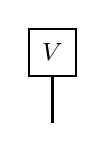
\begin{tikzpicture}[scale=0.3,thick] % , baseline = -3.5pt

\draw (1,1) rectangle (3,3);
\node[anchor=center] (text) at (2,2) {\small $V$};
\draw (2,-1)--(2,1) node[midway,right] {\tiny $\catvariable$};

\end{tikzpicture}
	\end{center}
\end{frame}













\end{document}